% !TeX spellcheck = en_US
\addsection{Combat}{\skills/attack.png}

\begin{multicols*}{2}

\pagetarget{Combat}{Combat}\index{Combat} with \textbf{Neutral Units} starts when a Hero moves to one of the \textbf{unvisited} Fields:
\begin{itemize}
  \item A Field with a Roman numeral signifying the \hyperlink{Difficulty Table}{type and number} of Neutral Units guarding that Field, or
\begin{expansion}[left=4mm]{navalbattles}
  \item A \pagelink{Creature Bank List}{Creature Bank Location}.
    In this case, follow the rules for \pagelink{Creature Banks Rules}{Combat against Creature Banks}.
\end{expansion}
\end{itemize}

Combat with \textbf{another player} can start in two ways:
\begin{itemize}
  \item You move into any Field containing one of their Heroes.
  \item You move into a Town or Settlement owned by them, see \pagelink{Siege Combat}{Siege Combat}.
\end{itemize}
Players are able to start multiple Combats during their Turn.

When a \pagelink{Secondary}{Secondary Hero} is attacked, they \textbf{may choose} to be \pagelink{Endcombat}{instantly defeated} instead of engaging in Combat, which helps to preserve the units.

\begin{center}
  \transparent{0.2}\includegraphics[width=0.6\linewidth]{\art/wyvern.png}
\end{center}

\pagetarget{Quick}{\subheader{Quick Combat}}\index{Quick Combat}
If your Hero's Level is higher than a Field's Difficulty when Combat against Neutral Units would begin, \textbf{no Combat} takes place.
The player is considered to have beaten the Neutral Units by default and gains no rewards from the Combat itself before Visiting the Field.

\vspace*{\fill}

\begin{center}
  % \vspace*{-1em}
  \includegraphics[width=\linewidth]{\art/rogue.jpg}
\end{center}
\end{multicols*}

\pagetarget{Combatsetup}{\subheader{Combat Setup}}
\begin{multicols*}{2}

\vspace*{-2em}
Combat is resolved on the 4×5 Combat Board, which consists of two Backlines and two Frontlines on opposite ends, and a middle row.
It can also be resolved on one of the \pagelink{Alternative Combat Boards}{alternative Boards}.
Follow these steps when Combat begins against \textbf{Neutral Units}:

\begin{itemize}[leftmargin=2.2em]
  \item Choose one of the Combat Board's sides as your own. Place up to 5 of your unit cards freely onto the Back and Frontlines of that side.
  \item Check the \hyperlink{Difficulty Table}{\textbf{Difficulty Table}} \iftoggle{printable}{(on the back cover)}{} and draw the corresponding number of Neutral Unit cards from their Decks.
  \item The Neutral Units are placed differently depending on the Game Mode:
  \item In \textbf{Clash} or \textbf{Alliance} Scenarios, the enemy player sitting to your right controls the Neutral Units and decides their placement. \svg{unit_ranged} units must be placed in the Backline if possible.
  \item \pagetarget{CombatAISetup}In \textbf{Campaign} or \textbf{Cooperative} Scenarios, Neutral Units are placed from left to right from the player's perspective.
First, place any \svg{unit_ranged} units in the Backline\index{Units Placement}.
Then, place any \svg{unit_ground} or \svg{unit_flying} units in the Frontline.
If there's not enough room to place a unit in its correct line, place them in the other one.
Units must be placed in \textbf{descending} Initiative\index{Initiative} order.
If there's a tie, place higher tier units first.
If there's still a tie, the players decide the order.
Check the \pagelink{AI Units}{\textbf{Combat against AI}} section for detailed instructions.
\end{itemize}

Unit setup when fighting \textbf{other players}:
\begin{itemize}[leftmargin=2.2em]
  \item The attacking player places up to 5 units on their chosen side of the Combat Board, followed by the defender.
  \item If the Combat takes place in a Town with a Citadel, the defender adds the \pagelink{Walls}{Wall, Gate and Arrow Tower} cards after placing their units.
\end{itemize}

\begin{center}
  \includegraphics[width=\linewidth]{\art/elf.jpg}
\end{center}
\end{multicols*}

\pagetarget{Combatterminology}{\subheader{Combat Terminology}}
\begin{multicols*}{2}
The following terms are used to describe effects and elements during Combat:\par
\textbf{Attacking Player} – The player who started the Combat.\par
\textbf{Defending Player} – The player whom Combat was started against.\par
\textbf{Activation} – A unit activates when it is next in the Initiative order.\par
\textbf{Adjacent Unit} – A unit is directly adjacent to another if it is one space away in a cardinal direction (nondiagonal).\par
\textbf{Combat Round} – A full cycle of all units of each player being activated.\par
\textbf{Combat Obstacles}\index{Combat Obstacles}\index{Obstacles, Combat} – Every card on the Combat Board is a Combat Obstacle.
They block the movement of all non-flying units.\smallskip\par
\begin{tikzpicture}[overlay]
  \node at (7, 0) {\includegraphics[width=0.2\linewidth]{\images/attack_die.png}};
\end{tikzpicture}\parbox{0.7\hsize}{\textbf{Attack Die}\index{Attack Die}\index{Dice} – A red Die whose results range from -1 to +1.
Roll the Die \textbf{whenever a unit attacks} and
add the result to the unit's Attack value.}\par\smallskip
\textbf{\pagetarget{Retaliate}{Retaliation Attack}} – If a unit survives an attack by an adjacent unit, it performs an attack back at that unit.
Each unit can perform \textbf{only 1} Retaliation Attack\index{Retaliation Attack} per Combat Round.
Retaliation Attacks function identically to normal attacks, but they cannot cause another Retaliation Attack.
Mark units which have performed a Retaliation Attack this Round with a Black Cube.\par
\textbf{\pagetarget{Paralysis}{Paralysis}}\index{Paralysis} \svg{paralysis} – Some effects place a Paralysis Token on units.
If a unit would activate with a Paralysis Token on it, \textbf{skip its activation} and remove the Token instead.
If the unit \textbf{is attacked or takes any damage} while having the Paralysis Token, remove it.
The Token does not prevent units from performing Retaliation Attacks.\par
\textbf{\pagetarget{Defend}{Defend}} \svg{defense} – units may choose to gain a Defense Token and end the activation instead of attacking.
When a unit with a Defense Token is attacked, make another roll with the attack Die after the initial attack roll.
If you roll a ``+1'', the defending unit gains an extra 1 Defense for this attack.
If a unit has a Defense Token at the start of its activation, discard it.
The unit cannot take another Defense Action during that activation.\par
\begin{expansion}{conflux}
  \textbf{\pagetarget{Elemental Damage}{Elemental Damage}} – If units deal elemental damage, they attack normally, but the resulting damage works similarly to \svg{damage} dealt by Spells and ignores the unit's \svg{defense}.
  Elemental damage does not count as damage from Spells.
\end{expansion}

\vspace*{\fill}
\begin{center}
  \hspace*{-2em}\transparent{0.2}\includegraphics[width=1.5\linewidth]{\art/storm_elemental.png}
\end{center}
\end{multicols*}

\pagetarget{combatround}{\subheader{Combat Round Structure}}
\begin{multicols*}{2}

Combat is divided into Rounds, during which all of the units participating in that Combat \textbf{activate once} in Initiative order.
After each unit has activated, a new Combat Round begins.
Combat lasts until all units on one side are eliminated, a player has to \textbf{Retreat}\index{Retreat} when fighting Neutral Units, or a player \textbf{surrenders} to another player.

Structure of a Combat Round:
\begin{itemize}[leftmargin=2.3em]
  \item Players activate their units in descending order of unit \pagelink{Initiative}{Initiative}. \textbf{If there's a tie}, alternate between attackers and defenders starting with an attacker.
  \item When a unit activates, place a Faction Cube on it to indicate it has been activated this Combat Round.
  \item Activated units may move and attack according to their \pagelink{Unittype}{type}. Neutral Units controlled by an opposing player must always attack if possible.
  \item Instead of attacking, a unit may \pagelink{Defend}{defend}.
  In Neutral Combat, the Neutral enemy units cannot defend, even when controlled by another player.
  \item Before a unit attacks, both players may \pagelink{CombatCards}{play cards}. Cards are resolved in the order in which players decide to play them.
  \item After a unit's attack has been declared and all cards have been played, roll the Attack Die.
    Modify the attacking unit's attack by the Die's result, then reduce it by the defending unit's Defense, and finally deal the rest as \pagelink{HP}{damage} to the defending unit.
  \item If the defending unit was adjacent to the attacker, it \pagelink{Retaliate}{retaliates} if it hasn't done so this Round.
  \item Keep activating units until they've all been activated once.
After the last unit's activation, the Combat Round ends.
\end{itemize}
\vspace*{\fill}

\subsection*{Campaign and Cooperative\\Combat}
During these game modes, all enemy units activate as described in the \pagelink{AI Units}{AI Rules section}.
\vspace*{\fill}

\subsection*{\pagetarget{CombatCards}{Using Cards During Combat}}
You may only use \textbf{one Spell per Combat Round}, unlike being able to play any number of other cards.
Ongoing \svg{ongoing} and \svg{activation} activation effects can be used only \textbf{when activating one of your units and before it attacks}.
Ongoing effects\index{Ongoing Effects} last until end of Combat or if the effect on the card is used up.\par
Instant \svg{instant} cards may be played \textbf{at any time} except between rolling the Attack Die and resolving damage unless otherwise stated.
Effects of increasing a unit's \svg{attack} (e.g. by the Statistics cards), expire whenever the first attack performed by that unit resolves or the activation ends, whichever comes first.
Increased \svg{defense} expires in a similar way.

\vspace*{\fill}

\subsection*{\pagetarget{Timelimit}{Combat Time Limits}}\index{Time Limit}
Combats against Neutral Units have a time limit of \textbf{one Combat Round}.
At the end of every Combat Round, you have an option to either \textbf{Retreat}\index{Retreat} or spend 1 \svg{movement} from the Hero that started the Combat in order to play another Round.
When you Retreat, end the Combat, and move the Hero that started the Combat back to the Field they \textbf{last Visited}.
Retreating has no other penalties.

\note{5}{Combats against Azure \svg{azure} Units, other players, or \pagelink{AIrules}{AI Heroes} have no time limit, and you cannot Retreat from them.}
\end{multicols*}

\pagetarget{Endcombat}{\subheader{End of Combat}}
\begin{multicols*}{2}
Combat against Neutrals has three possible outcomes:
\begin{itemize}
  \item \textbf{Victory:} All Neutral Units are defeated.
  \item \textbf{Retreat:} The player runs out of time or loses all combating units, but still has units in their unit Deck.
  \item \textbf{Defeat:} The player loses all combating units and doesn't have any units in their unit Deck.
\end{itemize}

Combat against another player's Hero has two possible outcomes:
\begin{itemize}
 \item \textbf{Victory/Defeat:} If all units on one side are defeated, the side with any surviving units is the winner, the other side is defeated.
 \item \textbf{Surrender:} Instead of activating one of their units, a Hero can decide to surrender to the other player's Hero by paying them 10 \svg{gold} to prevent their army from being defeated. In this case, Combat ends immediately without having a winning or defeated Hero.
\end{itemize}

When Combat ends, all damage is healed from all surviving units. Move any player-owned units back to their unit Deck and discard any leftover enemy Neutral Units. Depending on the type and result of the Combat, players must resolve the following consequences for themselves:

A \textbf{Winning Hero} gets \pagelink{Combatexperience}{Experience}, if it was the Main Hero. If it was the attacker, they must Visit the Field where the Combat took place.\par
A \textbf{Retreating Hero} from a Combat with Neutral Units has to move back to the last visited Field on the map (without Visiting that Field).\par
A \textbf{defeated Main Hero} has to move to a friendly Town or Settlement. If they were defeated by another player's Hero, they gain 1~\svg{morale_negative} and have to pay 5 \svg{gold} to the winning Hero. Furthermore, they give a \pagelink{End}{Faction Cube} to the winning player. Defeating a Main Hero may cause \pagelink{End}{Player Elimination}.\par
A \textbf{defeated Secondary Hero} (even instantly defeated without combat) is removed from the map. If defeated by another player's Hero they also get a Faction Cube.\par
A \textbf{Surrendering Hero} doesn't count as defeated. Move a surrendering Main Hero to a town or settlement, or remove a Secondary Hero from the map as if they had been defeated. The other player neither gets Experience nor Faction Cubes.\par
Remember to receive the starting units of the chosen Scenario for free each time your unit Deck is empty after a Combat.

\subsection*{\pagetarget{Combatexperience}{Combat Experience}}

Winning Combat with your Main Hero usually grants them Experience\index{Experience}.
If either the Difficulty of the Neutral Field or the Level of a defeated enemy Main Hero was \textbf{equal} to your Level, gain 1 \svg{experience}.
If they were \textbf{higher} than your Level, gain 2 \svg{experience}.
Winning a Neutral Combat against a Neutral Azure \svg{azure} Unit grants your Hero Level VII \textbf{immediately}.
If you ever gain multiple Levels at the same time, resolve their effects in order.
Level ups must be resolved before Visiting the Field where the Combat happened.\par
Secondary Heroes cannot ever gain Experience.
You also do not gain Experience from \textbf{defeating} a Secondary Hero, or if an enemy Hero \textbf{surrenders} to you.

\vspace*{\fill}
\begin{center}
  \transparent{0.2}\includegraphics[width=0.7\linewidth]{\art/basilisk.png}
\end{center}
\end{multicols*}

\clearpage

\subheader{Combat Example}

\begin{multicols*}{2}
\textit{Bob's Zombies are about to attack Alice's Griffins.
As Bob announces the attack, both players now have a chance to modify the Attack or Defense of their own unit by playing any number of \svg{instant} cards that increase an attacking unit's \svg{attack} or a defending unit's \svg{defense}.}\par
\textit{Bob decides to play a +1 Attack card, increasing the Zombies' attack from 2 to 3.
Alice responds by playing a +1 Defense card, increasing the Griffins' Defense from 0 to 1.
They would both be permitted to play any number of additional cards in any order, but they decide to stop after playing these cards.}\par

\includegraphics[width=\linewidth]{\examples/zombies_attack_griffins.png}

\textit{After all cards for the attack have been played, the Attack Die is thrown to further modify the amount of damage the attacking unit deals.
Bob throws a +1.
This increases the Zombies' attack from 3 to 4, which is then reduced by the Griffins' Defense of 1. Therefore, 3 damage \svg{damage} is placed on the Griffins. Since they have a HP \svg{health_points} of 4, they are not flipped over to their ``Few'' side.}\par
\columnbreak
\textit{The Griffins do not have a Black Cube on them, therefore they now start a Retaliation Attack.
The Cube would now normally be placed on them, however their Special \svg{unit_retaliate} Ability indicates that they may retaliate any number of times so the Cube is not placed.}\par
\textit{Both players are allowed to modify the Statistics of their units again during the Retaliation Attack.
The previously played Attack and Defense cards no longer have any effect.}

\vfill

{\transparent{0.2}\hspace{-1em}\includegraphics[width=1.7\linewidth]{\art/minotaur.png}}

\end{multicols*}

\clearpage

\pagetarget{Siege Combat}{\subheader{Siege Combat}}
\begin{multicols*}{2}
When an enemy Hero attacks your Town or Settlement and your Hero is not present on that Field, you may immediately \textbf{pay 8 \svg{gold} to defend with only your units}.
You cannot use your Deck during this Combat, as your Main Hero is not present.
Paying this Gold represents the cost of transporting the army there.

When you defend a Town \textbf{without a Citadel}, resolve Combat normally on the standard Combat Board.
Defending a Settlement follows the same rules as defending a Town without a Citadel.

\vspace{0.5em}
\note{3.5}{\textbf{Note:} you cannot surrender when defending your Faction Town.}\par

\pagetarget{Walls}{\subsection*{Defending a Town with a\\Citadel}}\index{Walls and Gate}
When you defend your Town and it has a Citadel, you add the 3~Wall and 1~Gate Obstacles in any order to the middle row of the Combat Board after placing your units.
\textbf{Don't use Walls and Gate} if you defend an enemy Town, which you've conquered before, \textbf{not even} if it is a Town with a Citadel.
The Gate Card is \textbf{not an Obstacle} to the defending player.
Defending units may move through the Gate and may stop on it.

Walls \pagelink{Walls protection}{protect defending units behind them}.

The Wall and Gate Cards can be destroyed by any adjacent \svg{unit_ground} or \svg{unit_flying} unit's attack, even by your own defending units.
These attacks don't count as normal attacks: They are always successful and don't activate any of the attacking unit's \svg{unit_attack} abilities, and you cannot play any cards or throw the Attack Die to affect the attack's result.

\vspace*{\fill}
\columnbreak

\begin{center}
  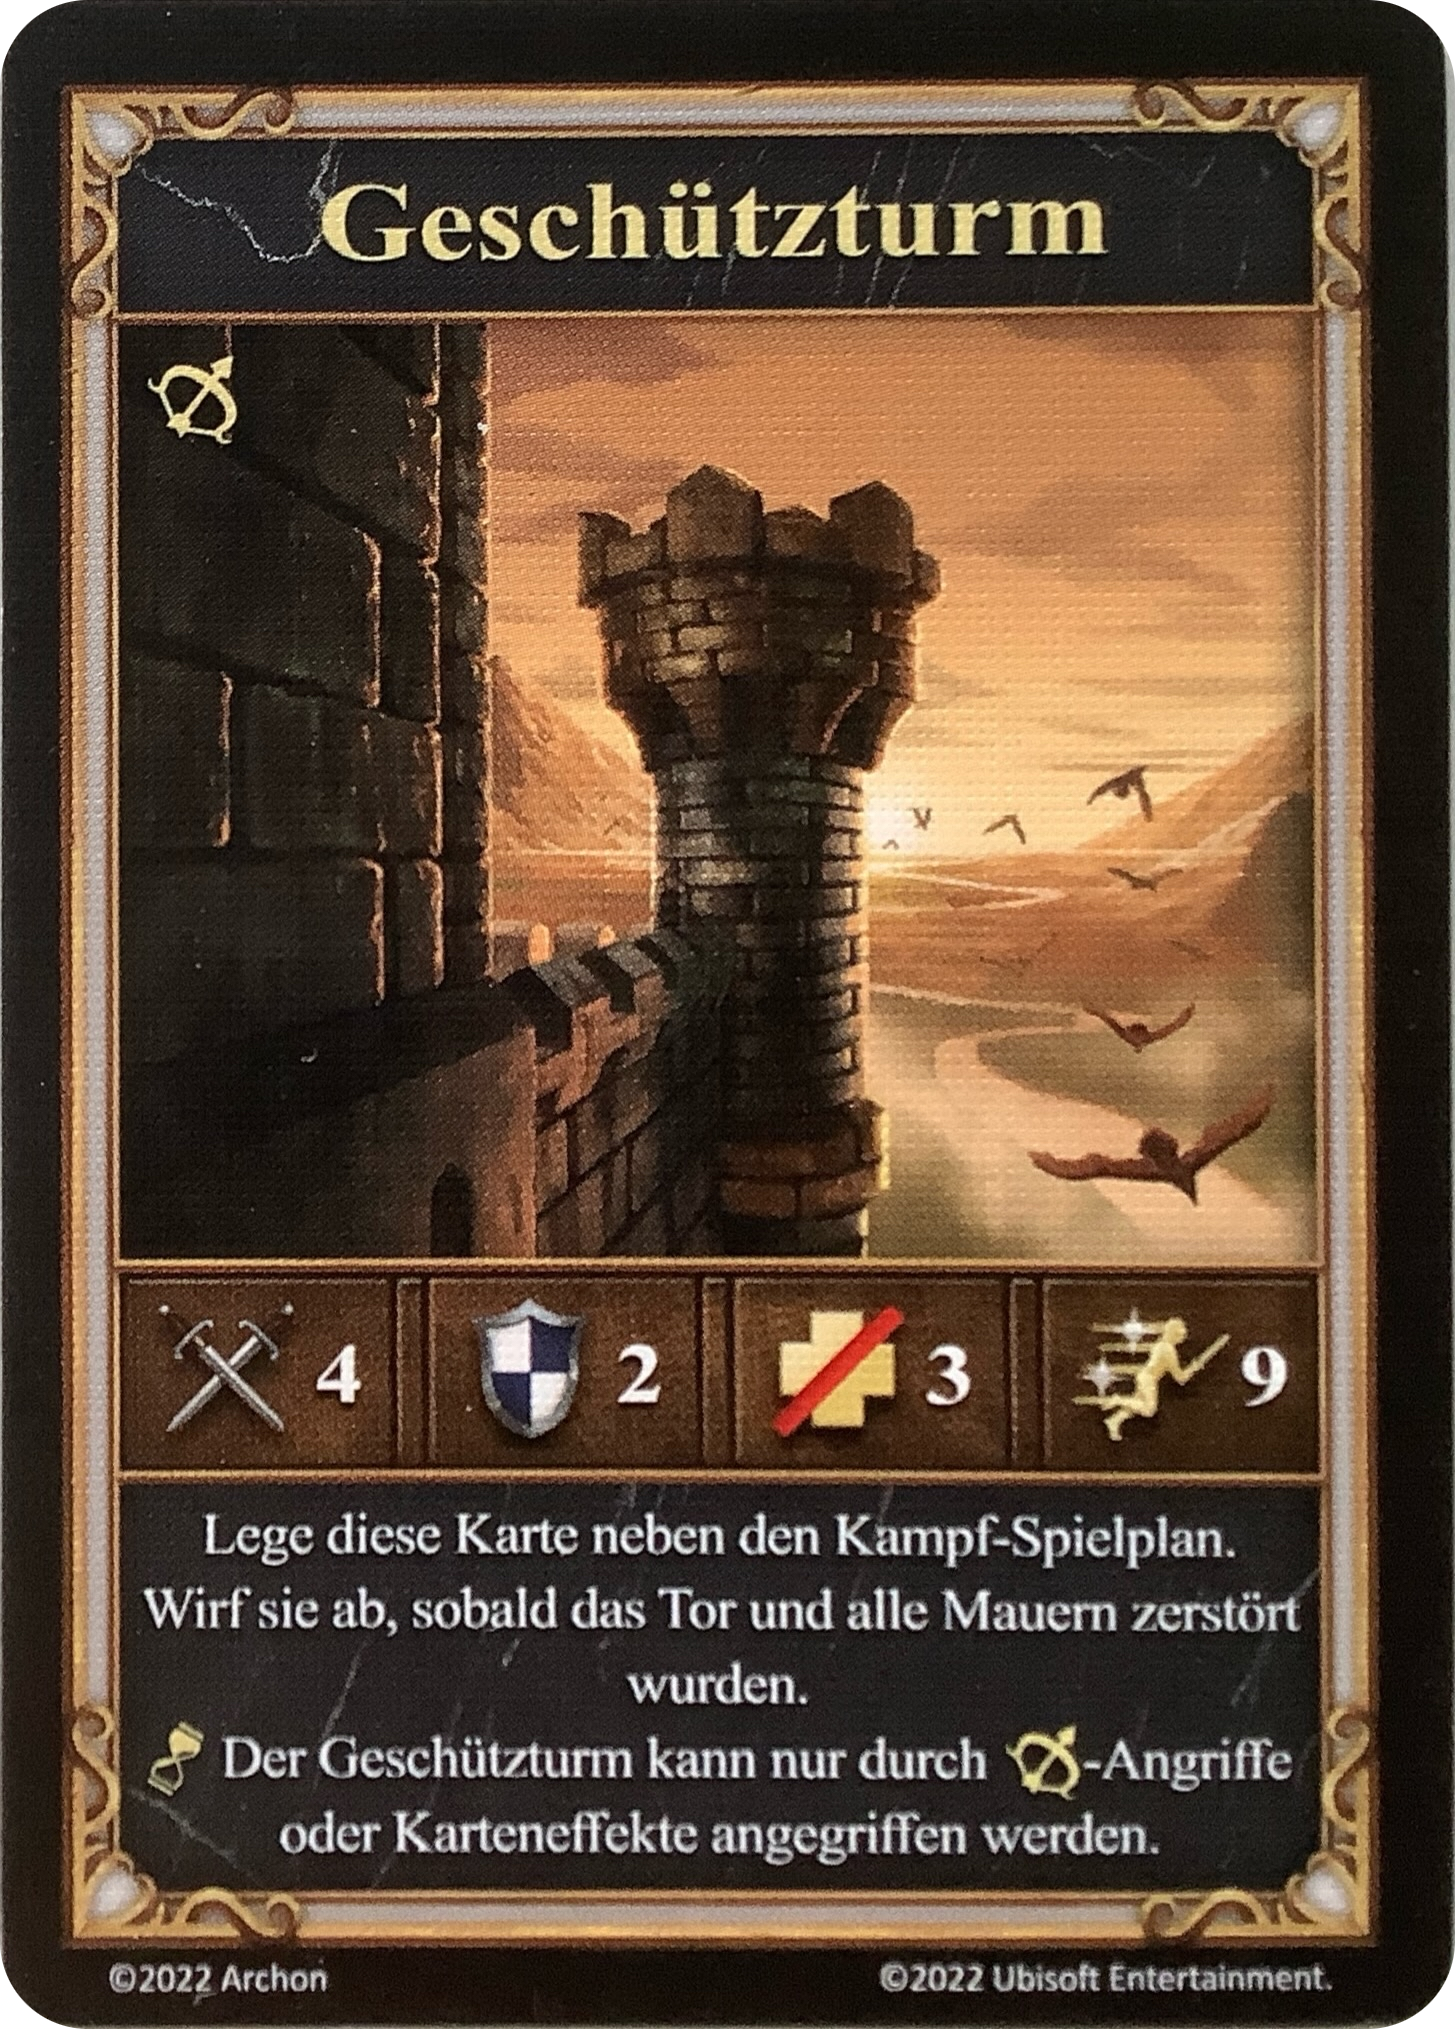
\includegraphics[width=0.6\linewidth]{\cards/arrow_tower.png}
\end{center}
The defender also gains the Arrow Tower\index{Arrow Tower} unit card which is placed next to the Combat Board.
It acts like a Ranged \svg{unit_ranged} unit, except that it is not affected by anything related to its positioning.
For example, it never gets ranged penalty against enemy units and vice versa.
Only Ranged attacks and card effects can destroy the Arrow Tower, but it is instantly destroyed when all Walls and the Gate are destroyed.
The attacker doesn't need to destroy it to win the Combat.

In a siege against AI, the Arrow Tower follows the priority rules like a Silver \svg{silver} unit.
However, if there are multiple equally valid targets, it will attack the target closest to being destroyed (the smallest difference between \svg{health_points} and current \svg{damage}).

\vspace*{\fill}
\begin{center}
  \transparent{0.2}\includegraphics[width=0.9\linewidth]{\art/coin.png}
\end{center}
\end{multicols*}

\newpage
\begin{multicols}{2}
\subsection*{\pagetarget{Walls protection}{Protection} from \svg[15]{unit_ranged} Attacks}

Defending units standing on their own side and \textbf{in the same column} as a non-destroyed Wall or Gate gain protection from \svg{unit_ranged} attacks.
If they are targeted by a \svg{unit_ranged} attack performed from the opponent's side of the Combat Board, \textbf{reduce the attack's damage by 1}.
\vspace*{\fill}

\begin{center}
  \transparent{0.15}\includegraphics[width=0.7\linewidth]{\art/lions_shield_of_courage.png}
\end{center}
\end{multicols}

\begin{multicols}{2}
\vspace*{\fill}
\includegraphics[width=\linewidth]{\examples/ranged_protected.png}
{\textit{When the Halberdiers are behind a non-destroyed Gate, they \textbf{are protected} when attacked from the opponent's side of the Combat Board.
  The \svg{unit_ranged} attack damage of Evil Eyes is \textbf{reduced by 1}.}}
\columnbreak

\vspace*{\fill}
\includegraphics[width=\linewidth]{\examples/ranged_unprotected.png}
{\textit{Because the Halberdiers are not behind a non-destroyed Wall, \textbf{protection doesn't work}.
  Evil Eyes attack \textbf{without penalty}.}}
\newline\newline
\end{multicols}
\newpage

\begin{multicols*}{2}

\pagetarget{Alternative Combat Boards}{\subheader{Alternative Combat Boards}}
\begin{expansion}{navalbattles}
  As an \textbf{optional rule}, you can use the \textbf{Naval Battle Board} for combats at sea locations.
  This Board removes the two middle spaces, requiring Ground \svg{unit_ground} units to navigate around them while Flying \svg{unit_flying} units can move over them but cannot end their movement there.

  \begin{center}
    \includegraphics[width=1.05\linewidth]{\images/naval_combat.png}
  \end{center}
\end{expansion}

\vspace{2em}
\begin{expansion}{battlefield}
  As an \textbf{optional rule}, you can use the \textbf{Battlefield Board} for combats between players in regular games.
  You can also use it for Neutral Combats, though this is not recommended.
  Refer to the \pagelink{Battlefield Combat}{Battlefield section} for the rule changes regarding this Combat type.

  \begin{center}
    \includegraphics[width=1.05\linewidth]{\images/battlefield-board.png}
  \end{center}
\end{expansion}
\vfill

\begin{center}
  \includegraphics[width=1.05\linewidth]{\art/rust_dragon.jpg}
\end{center}

\end{multicols*}
